%% generated by python/export_lever_figure.py
%% sweep: 2026-10-02-paper at commit 259ce29
%% aggregate test relative error, T=1, Adam, Legendre; every seed drawn,
% the curve is the geometric mean; unconstrained model at x=12.3
%   ELM ResNN       D=0 0.13108  D=11 0.12668  unconstrained 0.12768  (10 seeds)
%   ELM hamiltonian D=0 0.13299  D=11 0.14907  unconstrained 0.13147  (10 seeds)
%   CDR ResNN       D=0 0.00650  D=11 0.00481  unconstrained 0.00466  (10 seeds)
%   CDR hamiltonian D=0 0.00662  D=11 0.00503  unconstrained 0.00399  (10 seeds)
%   DCR ResNN       D=0 0.06193  D=11 0.04799  unconstrained 0.08696  (10 seeds)
%   DCR hamiltonian D=0 0.07155  D=11 0.05081  unconstrained 0.09254  (10 seeds)
\documentclass[tikz]{standalone}
\usepackage{pgfplots}
\usepgfplotslibrary{groupplots}
\pgfplotsset{compat=1.18}
\definecolor{mycolor3}{rgb}{0.0,0.0,1.0}
\definecolor{mycolor5}{rgb}{1.0,0.03,0.0}
\begin{document}
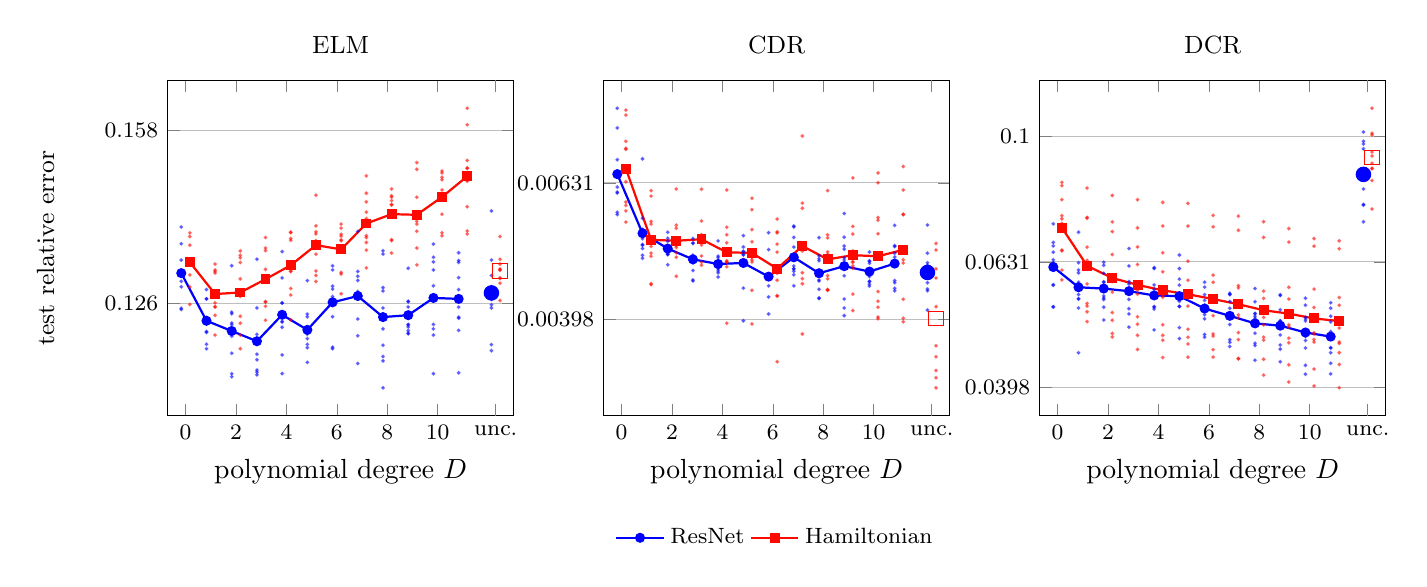
\begin{tikzpicture}
\begin{groupplot}[group style={group size=3 by 1,horizontal sep=1.15cm},
  width=2.35in,height=2.3in,ymode=log,
  log ticks with fixed point,
  xlabel={polynomial degree $D$},
  xtick={0,2,4,6,8,10},extra x ticks={12.3},extra x tick labels={unc.},
  extra x tick style={tick label style={font=\footnotesize}},
  xmin=-0.7,xmax=13.0,ymajorgrids,
  title style={font=\small},tick label style={font=\footnotesize},
  legend style={at={(0.5,-0.30)},anchor=north,legend columns=2,draw=none,
    fill=none,font=\footnotesize}]
\nextgroupplot[title={ELM}]
\addplot[only marks,mark=*,mark size=0.5pt,color=mycolor3,opacity=0.45,forget plot] coordinates {(-0.17,0.139363) (-0.17,0.125122) (-0.17,0.129666) (-0.17,0.136301) (-0.17,0.131390) (-0.17,0.133368) (-0.17,0.124895) (-0.17,0.131438) (-0.17,0.131264) (-0.17,0.128716) (0.83,0.122640) (0.83,0.118574) (0.83,0.128248) (0.83,0.126702) (0.83,0.123577) (0.83,0.126658) (0.83,0.121172) (0.83,0.119273) (0.83,0.122691) (0.83,0.121298) (1.83,0.121450) (1.83,0.124468) (1.83,0.124201) (1.83,0.122414) (1.83,0.132392) (1.83,0.122684) (1.83,0.114689) (1.83,0.117853) (1.83,0.120544) (1.83,0.114236) (2.83,0.114536) (2.83,0.120840) (2.83,0.117703) (2.83,0.133523) (2.83,0.119700) (2.83,0.114930) (2.83,0.116851) (2.83,0.125165) (2.83,0.115259) (2.83,0.120203) (3.83,0.122832) (3.83,0.126013) (3.83,0.125963) (3.83,0.130252) (3.83,0.124293) (3.83,0.114729) (3.83,0.122957) (3.83,0.134891) (3.83,0.117591) (3.83,0.121993) (4.83,0.116436) (4.83,0.124157) (4.83,0.120165) (4.83,0.123702) (4.83,0.120872) (4.83,0.121694) (4.83,0.119251) (4.83,0.129784) (4.83,0.118724) (4.83,0.121445) (5.83,0.123713) (5.83,0.118814) (5.83,0.125903) (5.83,0.131645) (5.83,0.118569) (5.83,0.127062) (5.83,0.128832) (5.83,0.126604) (5.83,0.128325) (5.83,0.132360) (6.83,0.130530) (6.83,0.116263) (6.83,0.129820) (6.83,0.138550) (6.83,0.123340) (6.83,0.131380) (6.83,0.120625) (6.83,0.127920) (6.83,0.126955) (6.83,0.127598) (7.83,0.128585) (7.83,0.112569) (7.83,0.121735) (7.83,0.128021) (7.83,0.119110) (7.83,0.135047) (7.83,0.125157) (7.83,0.134440) (7.83,0.116672) (7.83,0.117354) (8.83,0.122454) (8.83,0.120958) (8.83,0.121448) (8.83,0.126207) (8.83,0.125336) (8.83,0.131926) (8.83,0.121039) (8.83,0.122384) (8.83,0.122054) (8.83,0.126265) (9.83,0.114707) (9.83,0.133879) (9.83,0.120740) (9.83,0.131639) (9.83,0.133045) (9.83,0.136238) (9.83,0.121737) (9.83,0.122459) (9.83,0.126750) (9.83,0.128888) (10.83,0.125302) (10.83,0.128238) (10.83,0.123462) (10.83,0.130298) (10.83,0.121485) (10.83,0.133288) (10.83,0.114836) (10.83,0.134675) (10.83,0.123639) (10.83,0.132967)};
\addplot[color=mycolor3,mark=*,mark size=1.4pt,thick,forget plot] coordinates {(-0.17,0.131083) (0.83,0.123045) (1.83,0.121391) (2.83,0.119749) (3.83,0.124031) (4.83,0.121574) (5.83,0.126103) (6.83,0.127163) (7.83,0.123657) (8.83,0.123965) (9.83,0.126835) (10.83,0.126678)};
\addplot[only marks,mark=*,mark size=0.5pt,color=mycolor3,opacity=0.45,forget plot] coordinates {(12.13,0.125687) (12.13,0.125162) (12.13,0.130670) (12.13,0.128390) (12.13,0.118268) (12.13,0.133384) (12.13,0.126578) (12.13,0.142363) (12.13,0.128741) (12.13,0.119215)};
\addplot[color=mycolor3,mark=,mark size=2.6pt,only marks,forget plot] coordinates {(12.13,0.127680)};
\addplot[only marks,mark=*,mark size=0.5pt,color=mycolor5,opacity=0.45,forget plot] coordinates {(0.17,0.136032) (0.17,0.133219) (0.17,0.138271) (0.17,0.133358) (0.17,0.130771) (0.17,0.137615) (0.17,0.133318) (0.17,0.133409) (0.17,0.125739) (0.17,0.128719) (1.17,0.125385) (1.17,0.131387) (1.17,0.132666) (1.17,0.123941) (1.17,0.131101) (1.17,0.127296) (1.17,0.131638) (1.17,0.126013) (1.17,0.125316) (1.17,0.120740) (2.17,0.130089) (2.17,0.120730) (2.17,0.134221) (2.17,0.123780) (2.17,0.127086) (2.17,0.132948) (2.17,0.118577) (2.17,0.133785) (2.17,0.122658) (2.17,0.135007) (3.17,0.130236) (3.17,0.126184) (3.17,0.123139) (3.17,0.137421) (3.17,0.131741) (3.17,0.135062) (3.17,0.125434) (3.17,0.130194) (3.17,0.126177) (3.17,0.135523) (4.17,0.136930) (4.17,0.137242) (4.17,0.138330) (4.17,0.127327) (4.17,0.138406) (4.17,0.132853) (4.17,0.123205) (4.17,0.131388) (4.17,0.128432) (4.17,0.131423) (5.17,0.136642) (5.17,0.145366) (5.17,0.136857) (5.17,0.134415) (5.17,0.138480) (5.17,0.139583) (5.17,0.129636) (5.17,0.130689) (5.17,0.131461) (5.17,0.138094) (6.17,0.136851) (6.17,0.138015) (6.17,0.130930) (6.17,0.137666) (6.17,0.135061) (6.17,0.139904) (6.17,0.127541) (6.17,0.131225) (6.17,0.139142) (6.17,0.136994) (7.17,0.144109) (7.17,0.140936) (7.17,0.137435) (7.17,0.142140) (7.17,0.137789) (7.17,0.145751) (7.17,0.135148) (7.17,0.131989) (7.17,0.136527) (7.17,0.149150) (8.17,0.143550) (8.17,0.143533) (8.17,0.146592) (8.17,0.145018) (8.17,0.145269) (8.17,0.136859) (8.17,0.134629) (8.17,0.141396) (8.17,0.144323) (8.17,0.137026) (9.17,0.141978) (9.17,0.144975) (9.17,0.132530) (9.17,0.150455) (9.17,0.135516) (9.17,0.141305) (9.17,0.140430) (9.17,0.139904) (9.17,0.138578) (9.17,0.151808) (10.17,0.148385) (10.17,0.144859) (10.17,0.149734) (10.17,0.148862) (10.17,0.144800) (10.17,0.137743) (10.17,0.141752) (10.17,0.150126) (10.17,0.138306) (10.17,0.146398) (11.17,0.152242) (11.17,0.143179) (11.17,0.163154) (11.17,0.159635) (11.17,0.150693) (11.17,0.138084) (11.17,0.148086) (11.17,0.150657) (11.17,0.138628) (11.17,0.148285)};
\addplot[color=mycolor5,mark=square*,mark size=1.4pt,thick,forget plot] coordinates {(0.17,0.132994) (1.17,0.127493) (2.17,0.127755) (3.17,0.130030) (4.17,0.132461) (5.17,0.136048) (6.17,0.135277) (7.17,0.140008) (8.17,0.141764) (9.17,0.141634) (10.17,0.145032) (11.17,0.149067)};
\addplot[only marks,mark=*,mark size=0.5pt,color=mycolor5,opacity=0.45,forget plot] coordinates {(12.47,0.131818) (12.47,0.132656) (12.47,0.131587) (12.47,0.129337) (12.47,0.126393) (12.47,0.137625) (12.47,0.131686) (12.47,0.130141) (12.47,0.130272) (12.47,0.133504)};
\addplot[color=mycolor5,mark=square,mark size=2.6pt,only marks,forget plot] coordinates {(12.47,0.131473)};
\nextgroupplot[title={CDR}]
\addplot[only marks,mark=*,mark size=0.5pt,color=mycolor3,opacity=0.45,forget plot] coordinates {(-0.17,0.006480) (-0.17,0.005715) (-0.17,0.008118) (-0.17,0.005672) (-0.17,0.007599) (-0.17,0.006222) (-0.17,0.006100) (-0.17,0.006826) (-0.17,0.006565) (-0.17,0.006118) (0.83,0.005059) (0.83,0.005601) (0.83,0.004895) (0.83,0.005125) (0.83,0.004944) (0.83,0.005227) (0.83,0.005114) (0.83,0.005280) (0.83,0.006844) (0.83,0.005396) (1.83,0.004788) (1.83,0.004957) (1.83,0.005182) (1.83,0.004958) (1.83,0.004972) (1.83,0.005075) (1.83,0.005236) (1.83,0.005342) (1.83,0.005086) (1.83,0.004996) (2.83,0.004870) (2.83,0.004533) (2.83,0.005231) (2.83,0.004945) (2.83,0.005156) (2.83,0.004696) (2.83,0.004818) (2.83,0.005144) (2.83,0.004871) (2.83,0.004550) (3.83,0.004690) (3.83,0.004594) (3.83,0.005189) (3.83,0.004930) (3.83,0.004660) (3.83,0.004904) (3.83,0.004721) (3.83,0.004740) (3.83,0.004751) (3.83,0.004853) (4.83,0.004426) (4.83,0.004840) (4.83,0.004955) (4.83,0.004949) (4.83,0.004798) (4.83,0.003964) (4.83,0.005084) (4.83,0.004999) (4.83,0.005283) (4.83,0.005012) (5.83,0.004636) (5.83,0.004563) (5.83,0.004561) (5.83,0.004295) (5.83,0.004055) (5.83,0.004605) (5.83,0.004574) (5.83,0.004459) (5.83,0.005335) (5.83,0.005039) (6.83,0.005440) (6.83,0.004683) (6.83,0.004459) (6.83,0.005456) (6.83,0.004724) (6.83,0.005083) (6.83,0.004629) (6.83,0.004768) (6.83,0.004720) (6.83,0.005251) (7.83,0.004660) (7.83,0.004281) (7.83,0.005247) (7.83,0.004274) (7.83,0.004407) (7.83,0.004548) (7.83,0.004886) (7.83,0.004936) (7.83,0.004533) (7.83,0.004853) (8.83,0.004265) (8.83,0.004903) (8.83,0.004613) (8.83,0.005102) (8.83,0.005692) (8.83,0.004033) (8.83,0.004865) (8.83,0.005047) (8.83,0.004139) (8.83,0.005255) (9.83,0.004455) (9.83,0.004846) (9.83,0.004528) (9.83,0.004813) (9.83,0.004850) (9.83,0.004720) (9.83,0.004524) (9.83,0.004997) (9.83,0.004485) (9.83,0.004600) (10.83,0.004385) (10.83,0.004975) (10.83,0.004507) (10.83,0.005106) (10.83,0.004779) (10.83,0.004914) (10.83,0.005468) (10.83,0.005092) (10.83,0.004422) (10.83,0.004539)};
\addplot[color=mycolor3,mark=*,mark size=1.4pt,thick] coordinates {(-0.17,0.006501) (0.83,0.005325) (1.83,0.005057) (2.83,0.004876) (3.83,0.004800) (4.83,0.004817) (5.83,0.004600) (6.83,0.004910) (7.83,0.004653) (8.83,0.004765) (9.83,0.004679) (10.83,0.004807)};
\addplot[only marks,mark=*,mark size=0.5pt,color=mycolor3,opacity=0.45,forget plot] coordinates {(12.13,0.004735) (12.13,0.004979) (12.13,0.004579) (12.13,0.004507) (12.13,0.004413) (12.13,0.004386) (12.13,0.004109) (12.13,0.005475) (12.13,0.004781) (12.13,0.004820)};
\addplot[color=mycolor3,mark=,mark size=2.6pt,only marks,forget plot] coordinates {(12.13,0.004665)};
\addplot[only marks,mark=*,mark size=0.5pt,color=mycolor5,opacity=0.45,forget plot] coordinates {(0.17,0.005530) (0.17,0.006336) (0.17,0.008069) (0.17,0.005744) (0.17,0.005851) (0.17,0.007070) (0.17,0.007091) (0.17,0.007936) (0.17,0.005917) (0.17,0.007262) (1.17,0.004979) (1.17,0.004492) (1.17,0.005176) (1.17,0.004927) (1.17,0.004478) (1.17,0.005094) (1.17,0.005541) (1.17,0.006148) (1.17,0.005492) (1.17,0.006036) (2.17,0.005473) (2.17,0.005114) (2.17,0.005416) (2.17,0.005187) (2.17,0.004986) (2.17,0.005113) (2.17,0.005077) (2.17,0.004912) (2.17,0.004605) (2.17,0.006182) (3.17,0.005119) (3.17,0.006179) (3.17,0.005297) (3.17,0.004932) (3.17,0.004781) (3.17,0.005286) (3.17,0.004828) (3.17,0.005164) (3.17,0.005549) (3.17,0.005182) (4.17,0.004961) (4.17,0.004852) (4.17,0.005434) (4.17,0.004836) (4.17,0.005157) (4.17,0.004756) (4.17,0.004830) (4.17,0.006163) (4.17,0.003931) (4.17,0.005299) (5.17,0.005993) (5.17,0.005391) (5.17,0.005174) (5.17,0.004392) (5.17,0.003922) (5.17,0.005767) (5.17,0.004833) (5.17,0.004867) (5.17,0.004915) (5.17,0.004913) (6.17,0.004996) (6.17,0.004544) (6.17,0.005586) (6.17,0.004307) (6.17,0.003452) (6.17,0.005133) (6.17,0.004652) (6.17,0.004313) (6.17,0.005351) (6.17,0.005333) (7.17,0.007394) (7.17,0.005134) (7.17,0.005894) (7.17,0.005013) (7.17,0.003791) (7.17,0.005793) (7.17,0.004491) (7.17,0.004569) (7.17,0.005065) (7.17,0.004661) (8.17,0.004616) (8.17,0.004959) (8.17,0.006150) (8.17,0.004392) (8.17,0.004565) (8.17,0.005297) (8.17,0.004400) (8.17,0.004403) (8.17,0.005001) (8.17,0.005242) (9.17,0.006419) (9.17,0.004840) (9.17,0.004731) (9.17,0.004102) (9.17,0.005449) (9.17,0.005017) (9.17,0.004825) (9.17,0.005311) (9.17,0.004770) (9.17,0.004336) (10.17,0.006528) (10.17,0.006316) (10.17,0.005317) (10.17,0.004014) (10.17,0.003992) (10.17,0.004374) (10.17,0.004149) (10.17,0.005614) (10.17,0.005563) (10.17,0.004234) (11.17,0.006163) (11.17,0.003997) (11.17,0.005670) (11.17,0.004261) (11.17,0.005677) (11.17,0.003951) (11.17,0.004870) (11.17,0.004816) (11.17,0.006672) (11.17,0.005010)};
\addplot[color=mycolor5,mark=square*,mark size=1.4pt,thick] coordinates {(0.17,0.006623) (1.17,0.005208) (2.17,0.005192) (3.17,0.005218) (4.17,0.004993) (5.17,0.004983) (6.17,0.004725) (7.17,0.005101) (8.17,0.004876) (9.17,0.004945) (10.17,0.004927) (11.17,0.005035)};
\addplot[only marks,mark=*,mark size=0.5pt,color=mycolor5,opacity=0.45,forget plot] coordinates {(12.47,0.004157) (12.47,0.004723) (12.47,0.005032) (12.47,0.003352) (12.47,0.003270) (12.47,0.003643) (12.47,0.005145) (12.47,0.003510) (12.47,0.003161) (12.47,0.004578)};
\addplot[color=mycolor5,mark=square,mark size=2.6pt,only marks,forget plot] coordinates {(12.47,0.003993)};
\legend{ResNet,Hamiltonian}
\nextgroupplot[title={DCR}]
\addplot[only marks,mark=*,mark size=0.5pt,color=mycolor3,opacity=0.45,forget plot] coordinates {(-0.17,0.062963) (-0.17,0.065391) (-0.17,0.058048) (-0.17,0.053485) (-0.17,0.067772) (-0.17,0.072549) (-0.17,0.066920) (-0.17,0.057931) (-0.17,0.053552) (-0.17,0.063593) (0.83,0.062932) (0.83,0.055138) (0.83,0.053294) (0.83,0.055100) (0.83,0.061255) (0.83,0.070373) (0.83,0.058588) (0.83,0.055984) (0.83,0.045236) (0.83,0.060623) (1.83,0.060539) (1.83,0.058544) (1.83,0.053461) (1.83,0.054965) (1.83,0.062314) (1.83,0.063034) (1.83,0.055711) (1.83,0.055269) (1.83,0.050997) (1.83,0.058678) (2.83,0.058162) (2.83,0.056898) (2.83,0.052153) (2.83,0.053169) (2.83,0.062183) (2.83,0.066283) (2.83,0.055003) (2.83,0.056464) (2.83,0.049681) (2.83,0.058727) (3.83,0.057998) (3.83,0.055446) (3.83,0.053579) (3.83,0.053082) (3.83,0.061584) (3.83,0.061816) (3.83,0.053462) (3.83,0.056070) (3.83,0.049183) (3.83,0.057070) (4.83,0.059255) (4.83,0.054624) (4.83,0.053592) (4.83,0.047653) (4.83,0.061595) (4.83,0.064722) (4.83,0.053603) (4.83,0.057962) (4.83,0.049600) (4.83,0.056201) (5.83,0.057544) (5.83,0.053842) (5.83,0.051231) (5.83,0.047883) (5.83,0.058583) (5.83,0.051999) (5.83,0.052742) (5.83,0.054810) (5.83,0.048368) (5.83,0.055967) (6.83,0.056257) (6.83,0.047000) (6.83,0.050160) (6.83,0.046282) (6.83,0.054584) (6.83,0.052212) (6.83,0.053242) (6.83,0.055977) (6.83,0.047455) (6.83,0.056046) (7.83,0.054543) (7.83,0.046454) (7.83,0.048580) (7.83,0.044004) (7.83,0.052206) (7.83,0.052236) (7.83,0.051714) (7.83,0.057253) (7.83,0.046839) (7.83,0.051339) (8.83,0.055792) (8.83,0.046542) (8.83,0.045840) (8.83,0.043766) (8.83,0.050795) (8.83,0.052953) (8.83,0.050848) (8.83,0.055950) (8.83,0.048266) (8.83,0.050293) (9.83,0.053857) (9.83,0.047315) (9.83,0.048024) (9.83,0.043193) (9.83,0.050814) (9.83,0.051521) (9.83,0.046028) (9.83,0.055252) (9.83,0.041823) (9.83,0.051197) (10.83,0.054333) (10.83,0.045238) (10.83,0.046090) (10.83,0.043523) (10.83,0.048889) (10.83,0.051716) (10.83,0.046032) (10.83,0.053267) (10.83,0.041866) (10.83,0.050644)};
\addplot[color=mycolor3,mark=*,mark size=1.4pt,thick,forget plot] coordinates {(-0.17,0.061929) (0.83,0.057500) (1.83,0.057230) (2.83,0.056688) (3.83,0.055806) (4.83,0.055660) (5.83,0.053188) (6.83,0.051784) (7.83,0.050372) (8.83,0.049954) (9.83,0.048720) (10.83,0.047991)};
\addplot[only marks,mark=*,mark size=0.5pt,color=mycolor3,opacity=0.45,forget plot] coordinates {(12.13,0.082433) (12.13,0.097198) (12.13,0.095493) (12.13,0.073099) (12.13,0.101575) (12.13,0.098197) (12.13,0.077872) (12.13,0.085566) (12.13,0.085637) (12.13,0.077727)};
\addplot[color=mycolor3,mark=,mark size=2.6pt,only marks,forget plot] coordinates {(12.13,0.086965)};
\addplot[only marks,mark=*,mark size=0.5pt,color=mycolor5,opacity=0.45,forget plot] coordinates {(0.17,0.079293) (0.17,0.073924) (0.17,0.084476) (0.17,0.065890) (0.17,0.059065) (0.17,0.061248) (0.17,0.074777) (0.17,0.065748) (0.17,0.072660) (0.17,0.083444) (1.17,0.074069) (1.17,0.063458) (1.17,0.082712) (1.17,0.053681) (1.17,0.050711) (1.17,0.054191) (1.17,0.066608) (1.17,0.058215) (1.17,0.052569) (1.17,0.074277) (2.17,0.073074) (2.17,0.058731) (2.17,0.080509) (2.17,0.050949) (2.17,0.048555) (2.17,0.052416) (2.17,0.064847) (2.17,0.056491) (2.17,0.047940) (2.17,0.070530) (3.17,0.071487) (3.17,0.056901) (3.17,0.079282) (3.17,0.050225) (3.17,0.048213) (3.17,0.051615) (3.17,0.062499) (3.17,0.056076) (3.17,0.045792) (3.17,0.066672) (4.17,0.071978) (4.17,0.055462) (4.17,0.078487) (4.17,0.047347) (4.17,0.048211) (4.17,0.050133) (4.17,0.060885) (4.17,0.055783) (4.17,0.044453) (4.17,0.065265) (5.17,0.071959) (5.17,0.053668) (5.17,0.078208) (5.17,0.046710) (5.17,0.047873) (5.17,0.049305) (5.17,0.058995) (5.17,0.055253) (5.17,0.044507) (5.17,0.063282) (6.17,0.071770) (6.17,0.051822) (6.17,0.074844) (6.17,0.045757) (6.17,0.048079) (6.17,0.048472) (6.17,0.058565) (6.17,0.055168) (6.17,0.044523) (6.17,0.060111) (7.17,0.070855) (7.17,0.051409) (7.17,0.074639) (7.17,0.044228) (7.17,0.047473) (7.17,0.048707) (7.17,0.057394) (7.17,0.051959) (7.17,0.044291) (7.17,0.057849) (8.17,0.069020) (8.17,0.050121) (8.17,0.073124) (8.17,0.041671) (8.17,0.047369) (8.17,0.047911) (8.17,0.056686) (8.17,0.051500) (8.17,0.044168) (8.17,0.055199) (9.17,0.067860) (9.17,0.049714) (9.17,0.071304) (9.17,0.040636) (9.17,0.046919) (9.17,0.047706) (9.17,0.057491) (9.17,0.050121) (9.17,0.043284) (9.17,0.055073) (10.17,0.066850) (10.17,0.048655) (10.17,0.068735) (10.17,0.040060) (10.17,0.047491) (10.17,0.047039) (10.17,0.057114) (10.17,0.048465) (10.17,0.042611) (10.17,0.053387) (11.17,0.066235) (11.17,0.049529) (11.17,0.068171) (11.17,0.039783) (11.17,0.047048) (11.17,0.046809) (11.17,0.055397) (11.17,0.045254) (11.17,0.043342) (11.17,0.053847)};
\addplot[color=mycolor5,mark=square*,mark size=1.4pt,thick,forget plot] coordinates {(0.17,0.071554) (1.17,0.062211) (2.17,0.059487) (3.17,0.058007) (4.17,0.056861) (5.17,0.056045) (6.17,0.055073) (7.17,0.054041) (8.17,0.052858) (9.17,0.052203) (10.17,0.051290) (11.17,0.050808)};
\addplot[only marks,mark=*,mark size=0.5pt,color=mycolor5,opacity=0.45,forget plot] coordinates {(12.47,0.093062) (12.47,0.094395) (12.47,0.101085) (12.47,0.090576) (12.47,0.076611) (12.47,0.088939) (12.47,0.100446) (12.47,0.088774) (12.47,0.085036) (12.47,0.110813)};
\addplot[color=mycolor5,mark=square,mark size=2.6pt,only marks,forget plot] coordinates {(12.47,0.092538)};
\end{groupplot}
\node[anchor=south,rotate=90,font=\small] at ([xshift=-1.32cm]group c1r1.west) {test relative error};
\end{tikzpicture}
\end{document}
